\subsection{Dataset for Echo-aware processing}

\begin{frame}{Echo-aware Datasets}

    \begin{block}{\alert{Data} in audio signal processing}
        \begin{enumerate}
            \item are necessary for validating (and learning) models
            \item collecting real data is a not always possible
            \\\hspace{.3em} annotation and recording require expertise, equipment and \alert{time}
            \item dataset of real data cannot be easily shared
            \\\hspace{.3em} they do not generalize to different use-cases and scenarios (array, recording scenario)
            \item \alert{simulated data} are used instead: quantity, versatility, annotation easiness and ``quality''
        \end{enumerate}
    \end{block}

    \begin{block}{\alert{Echo-aware Data} in audio signal processing}
        \begin{description}
            \item[For SE:] strong echoes, but not annotated
            \\{\small\cite{szoke2019building,bertin2019voicehome,remaggi2016acoustic}}
            \item[For RooGE:] good geo. annotation, but no variety of acoustic scenarios
            \\{\small\cite{dokmanic2013acoustic,crocco2017uncalibrated,remaggi2019modeling}}
        \end{description}
    \end{block}

    \begin{center}
        \textcolor{myred}{A good echo-aware dataset should allow \textbf{SE}, \textbf{RooGE} and \textbf{AER}
        \\HOW?
        \\signal annotation \quad $\Longleftrightarrow$ \quad geometric annotation}
    \end{center}

\end{frame}

\subsection{\dechorate}

\begin{frame}[t]{\dechorate realization}

    \begin{block}{\dechorate: echo-aware dataset}
        Recorded Acoustic lab of Bar'Ilan (Shoebox)
        \\Annotated during confinement COVID-2020
        \\Collaboration with prof. Sharon Gannot and ing. Pinchas Tandeitnik
    \end{block}

    \only<2>{
    \begin{block}{Key features:}
        \begin{itemize}
            \item many acoustic environments (revolving panels)
            \item 6 nULA with 5 mics and 4 sound sources
            \item geometry annotated \& echo annotated
            \item measured RIRs $\overset{\text{matching}}{\longrightarrow}$ simulated RIRs
        \end{itemize}
    \end{block}
    }

    \vfill
    \only<1>{
        \begin{center}
            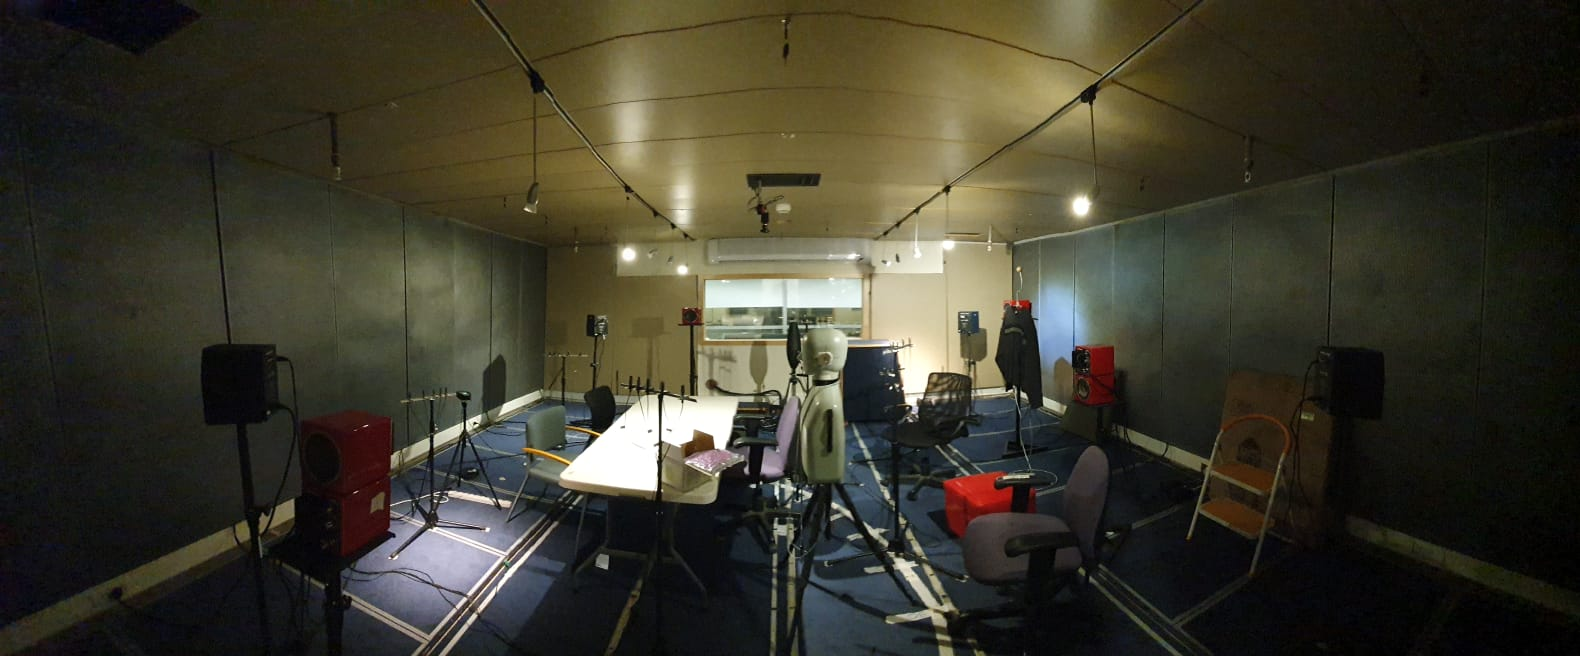
\includegraphics[trim={0 0 0 10em},clip,width=\textwidth]{figures/dechorate/fornitures.jpg}
        \end{center}
    }
    \only<2>{
        \begin{columns}[T,onlytextwidth]
            \begin{column}{0.3\textwidth}
                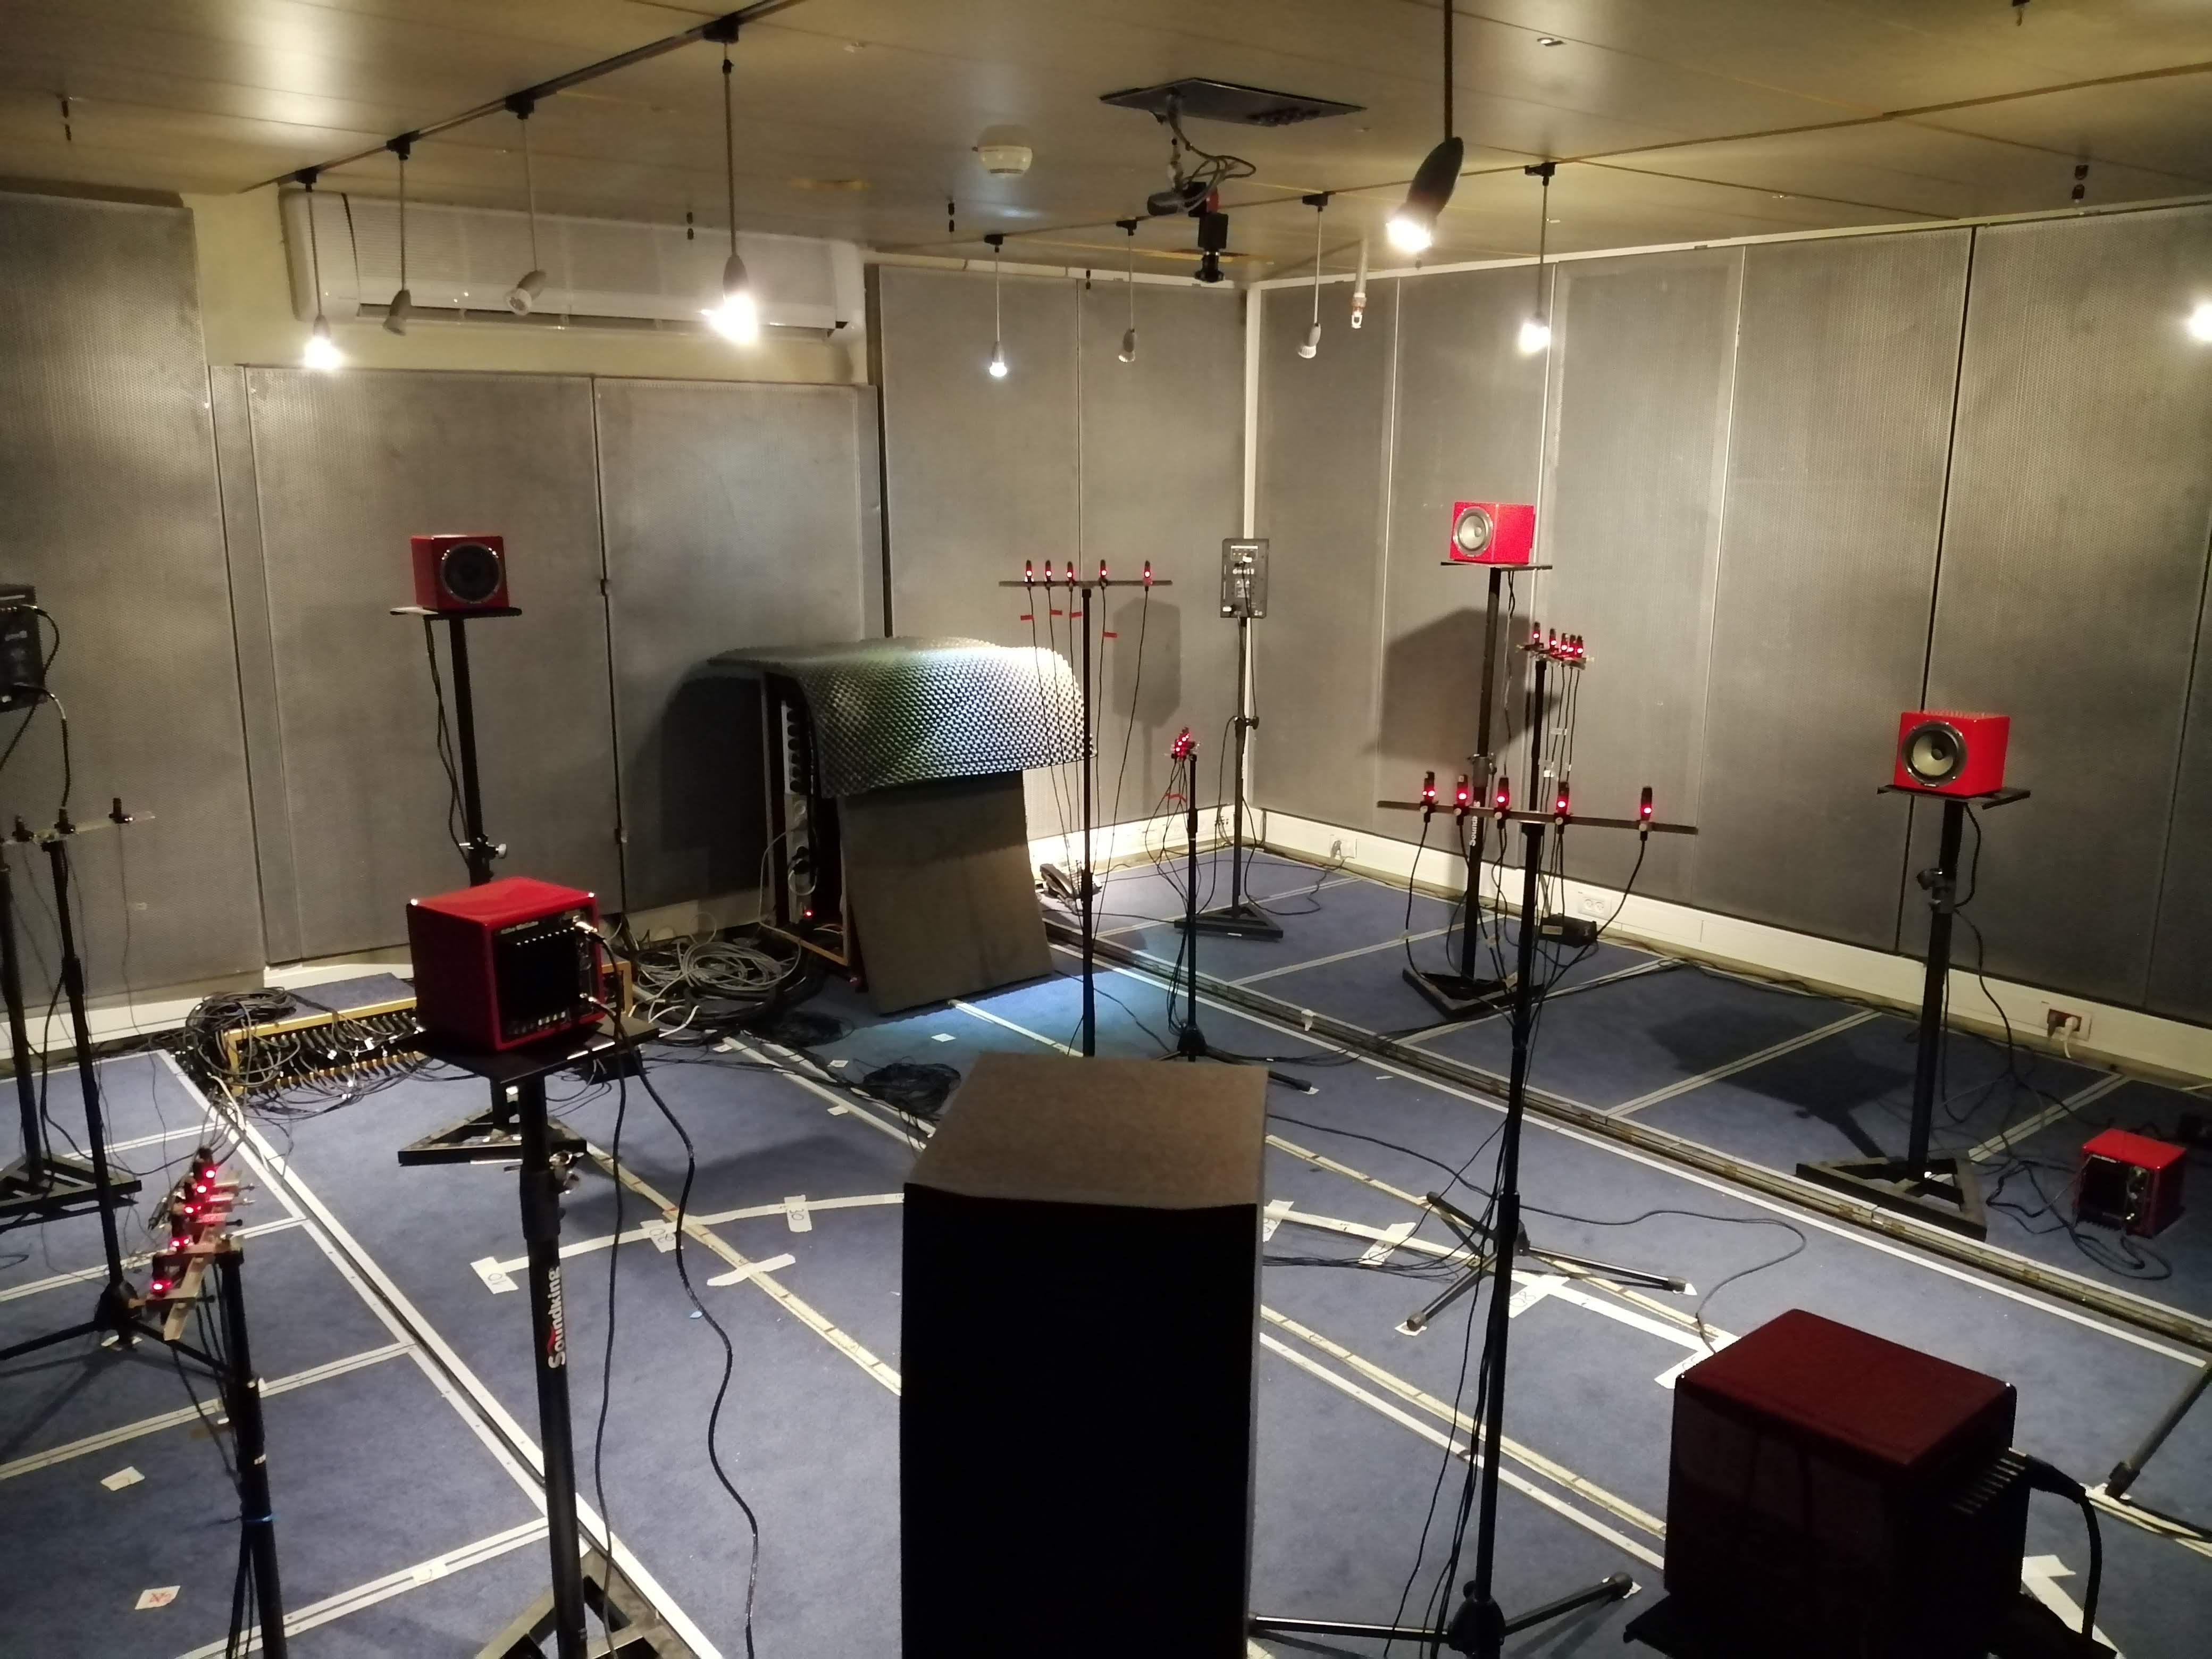
\includegraphics[width=\textwidth]{figures/dechorate/recording_setup}
            \end{column}\hfill
            \begin{column}{0.3\textwidth}
                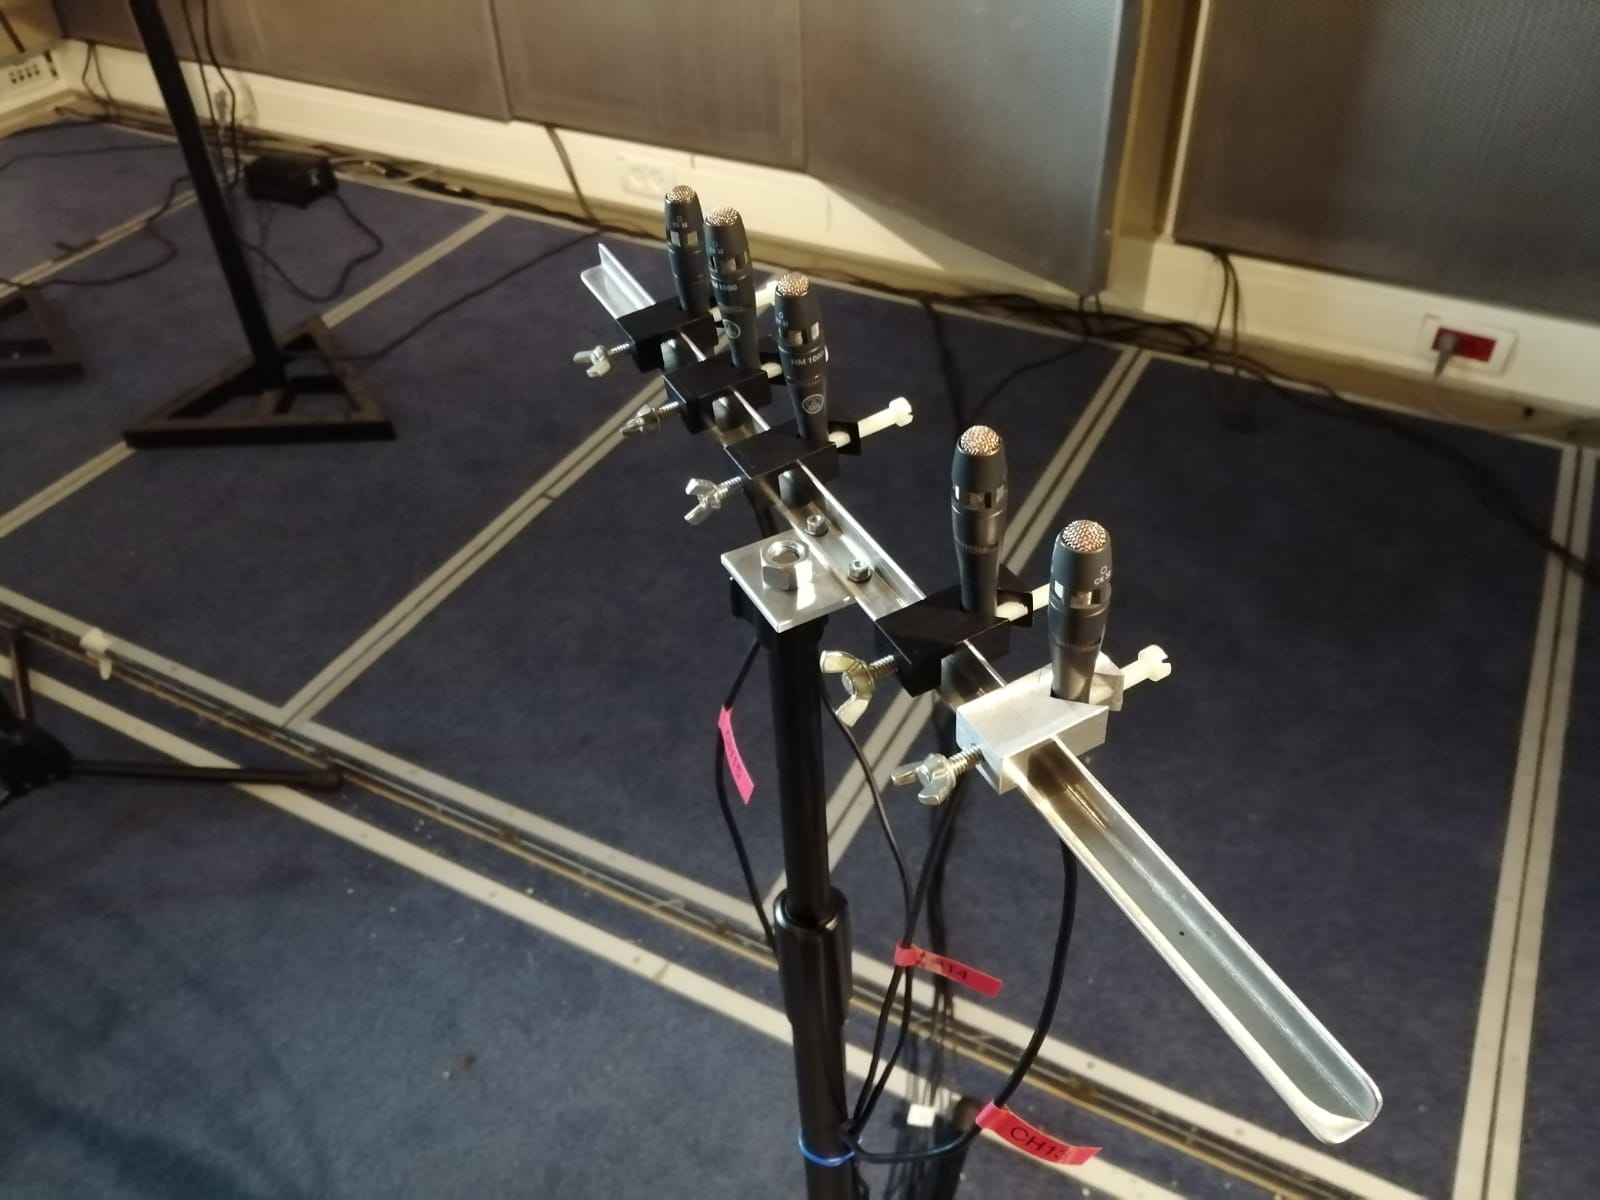
\includegraphics[width=\textwidth]{figures/dechorate/mic}
            \end{column}\hfill
            \begin{column}{0.3\textwidth}
                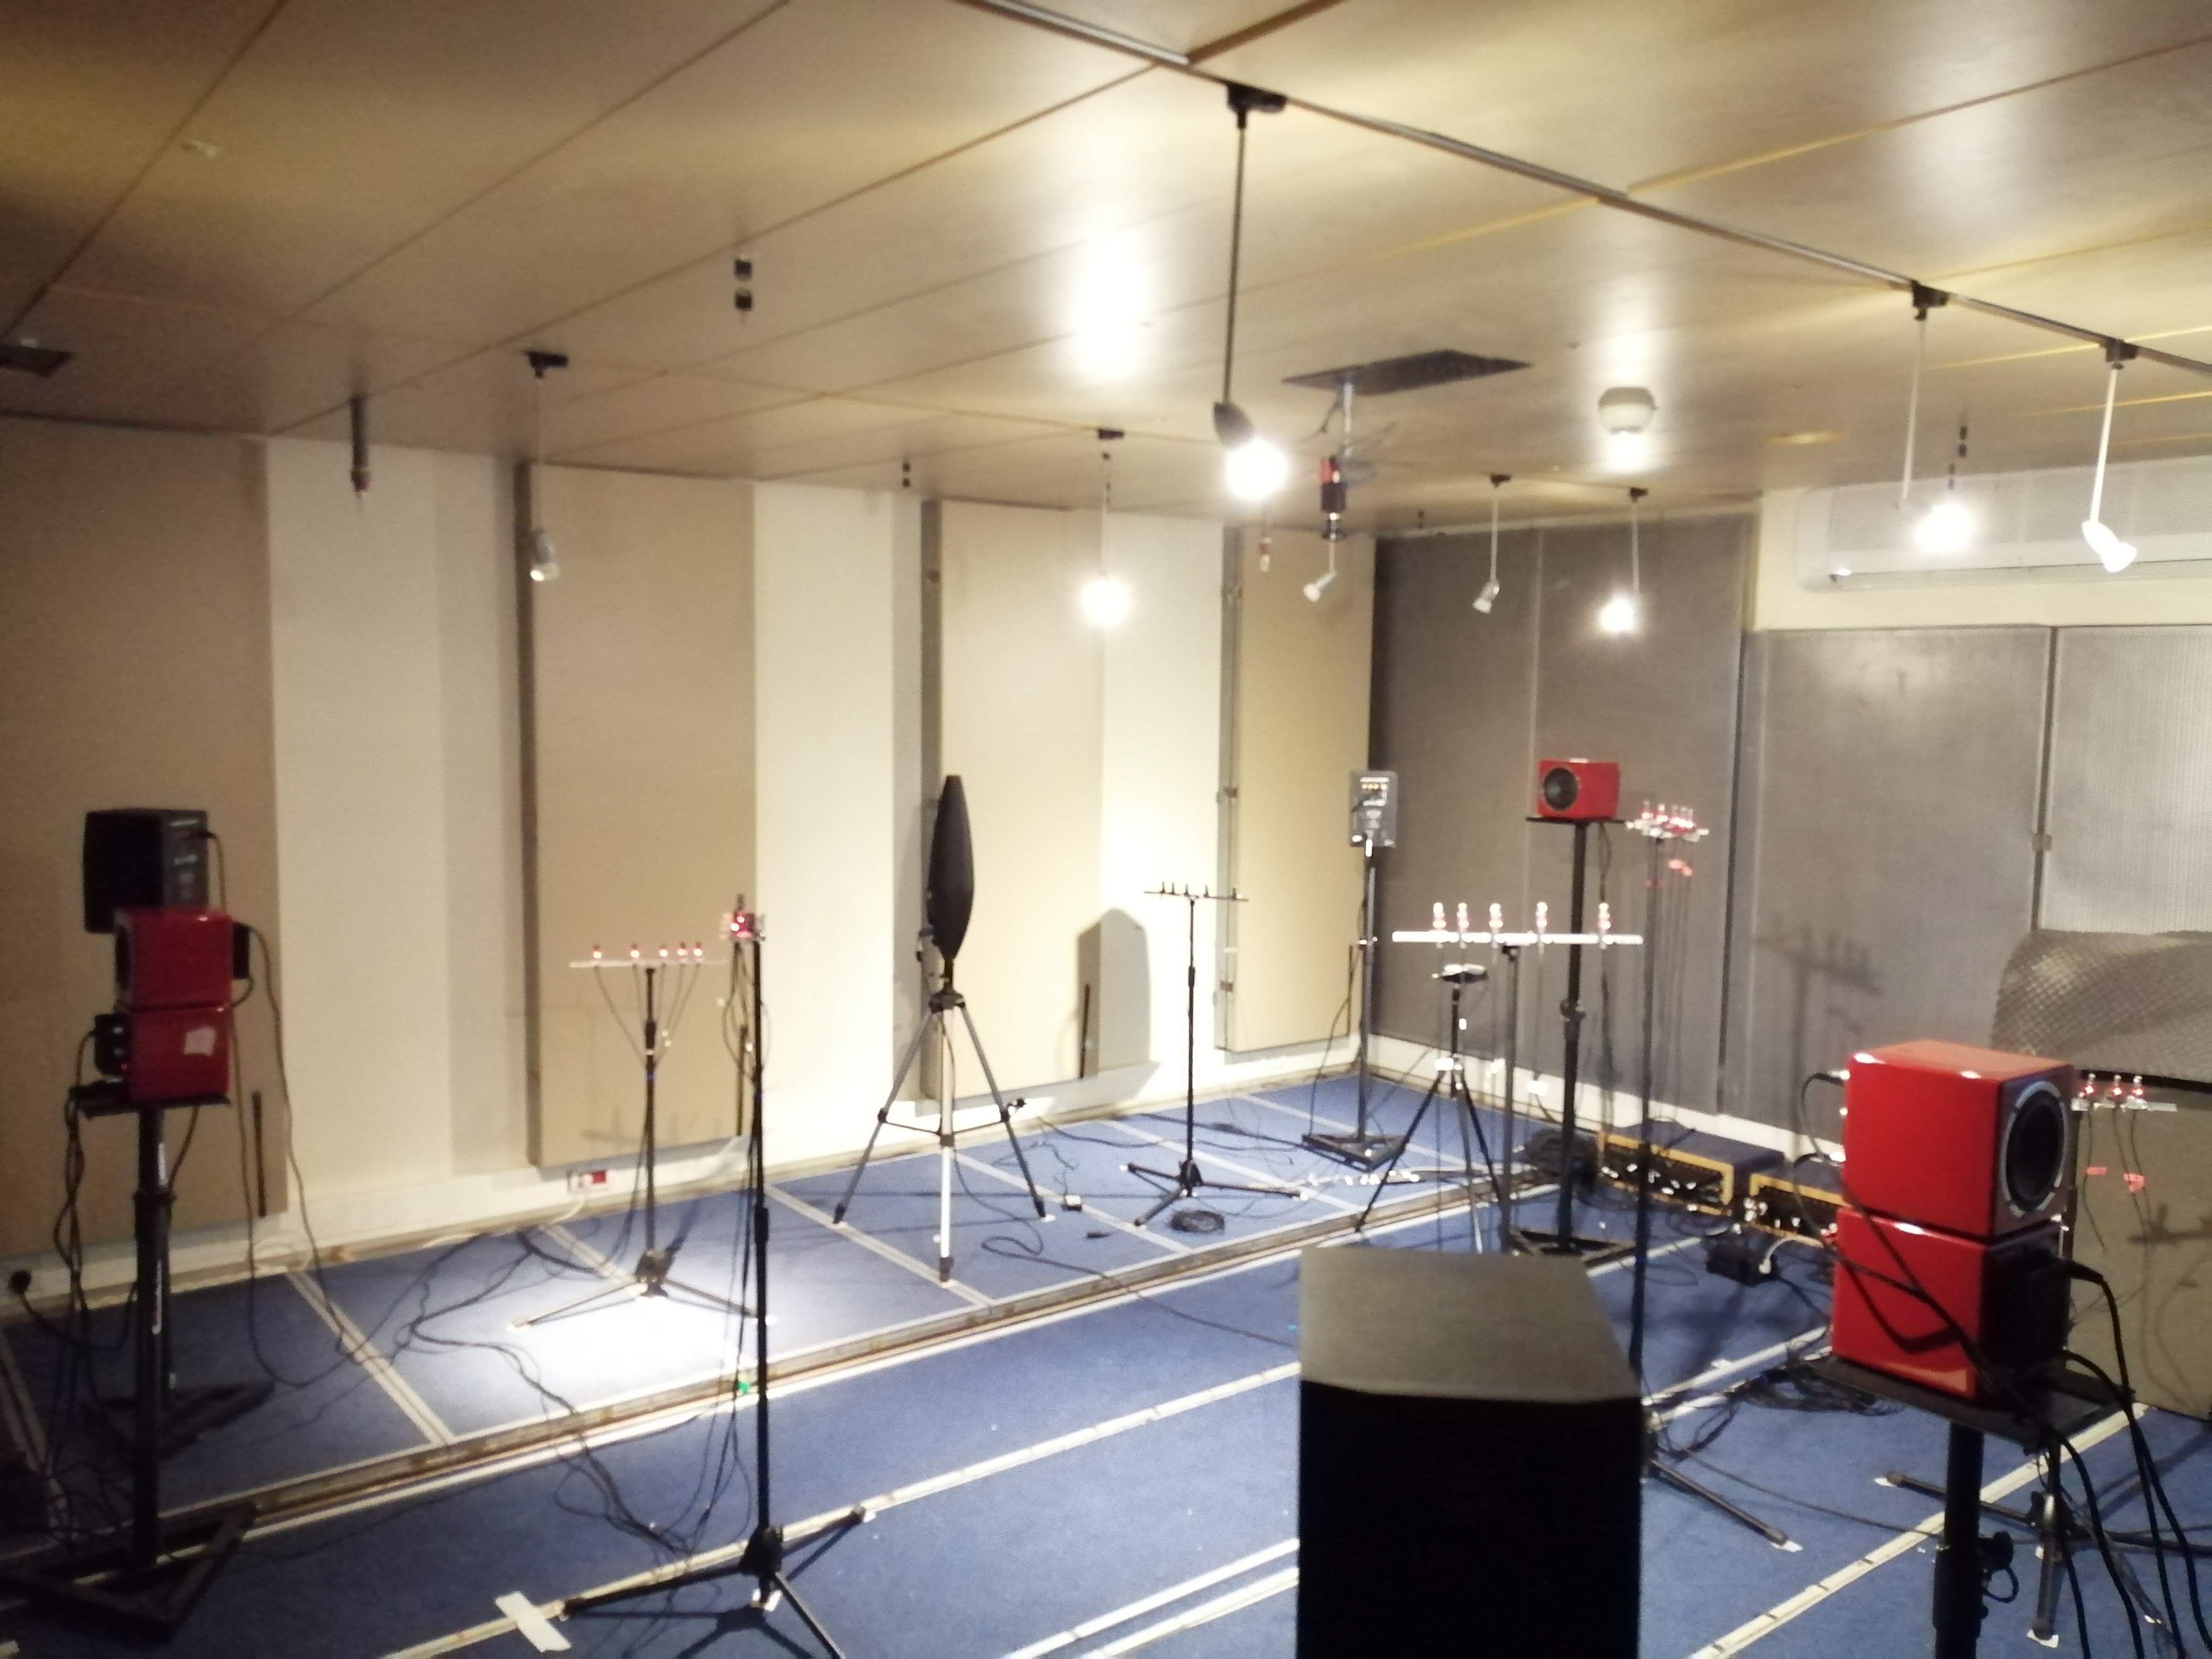
\includegraphics[width=\textwidth]{figures/dechorate/panels}
            \end{column}
        \end{columns}
    }

\end{frame}


\begin{frame}[t]{\dechorate --- Annotation}

    \begin{enumerate}
        \item RIR estimation with chirps signal~\cite{farina2007advancements,szoke2019building}
        \item IPS with beacon $\longrightarrow$ mic and src positioning ($\pm 2$ cm)
        \item GUI for echo annotation
        \\Skyline, Matched Filter, Assisted Peak Picking
        \item Refined position with Least Square optimization
        \item iterate including ceiling (perfectly flat)
    \end{enumerate}

    \vfill
    \only<2>{
        \begin{adjustbox}{minipage=.8\textwidth,margin=0pt \smallskipamount,center}
            \centering
            \small
            \begin{tabular*}{\linewidth}{@{\extracolsep{\fill}}lllll@{}}
                \toprule
                & Metrics      & $\mathtt{bIPS}$  & $\mathtt{dMDS}$ & $\mathtt{dcMDS}$          \\
                \midrule
                \multicolumn{1}{c}{\multirow{2}{*}{\rotatebox{90}{\footnotesize Geom.}}}
                &   Max.             & 0            & $6.1$          & $1.07$        \\
                &   Avg.$\pm$Std.    & 0            & $1.8\pm1.4$    & $0.39\pm0.2$  \\
                % \rule{0pt}{0.1em}\\
                \midrule
                \multicolumn{1}{c}{\multirow{2}{*}{\rotatebox{90}{\footnotesize Signal}}}
                &   Max.          & $5.86$         & $1.20$         & $1.86$       \\
                &   Avg.$\pm$Std. & $1.85\pm 1.5$  & $0.16\pm0.2$   & $0.41\pm0.3$ \\
                % \rule{0pt}{0.1em}\\
                \midrule
                \multicolumn{1}{c}{\multirow{3}{*}{\rotatebox{90}{\footnotesize Mismatch}}}
                &  GoM (1.0 ms)   & $97.9 \%$      & $93.4 \%$      & $98.1 \%$ \\
                &  GoM (0.1 ms)   & $26.6 \%$      & $44.8 \%$      & $53.1 \%$ \\
                &  GoM (0.05 ms)  & $12.5 \%$      & $14.4 \%$      & $30.2 \%$ \\
                \bottomrule
            \end{tabular*}

            \vspace{3mm}
            \textcolor{gray}{GoM = Goodness of Match ($\neq$ error, because no groundtruth)}
        \end{adjustbox}
    }

    \only<3>{
        \begin{center}
            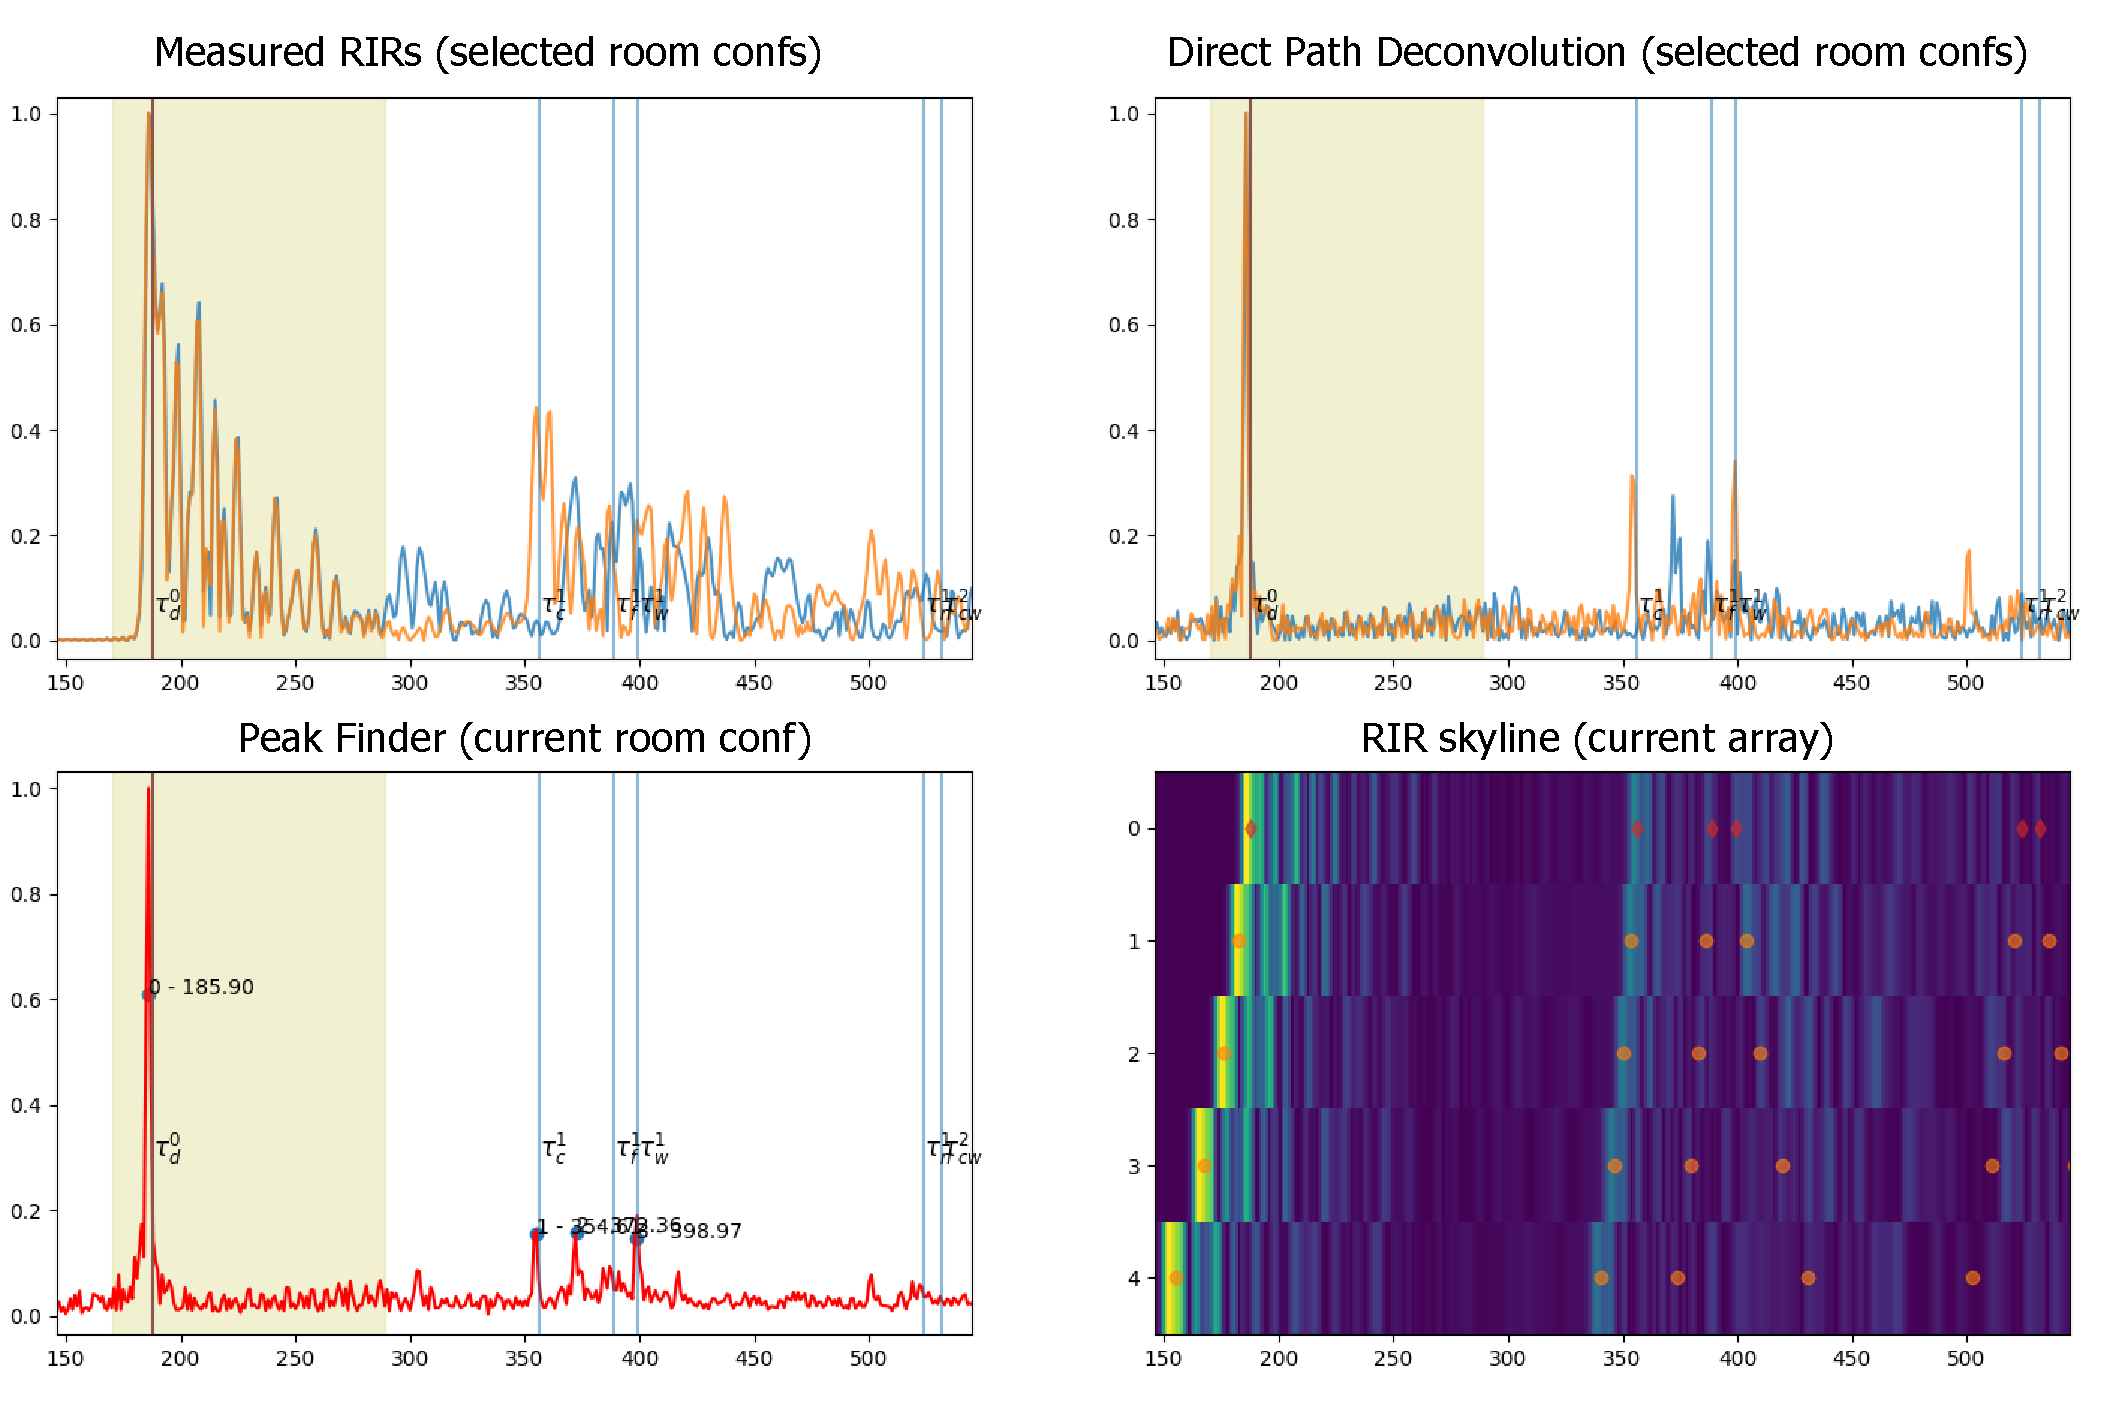
\includegraphics[width=.8\textwidth]{figures/dechorate/labeling_tool.pdf}
        \end{center}
    }
\end{frame}

\begin{frame}{\dechorate --- Annotation}
    \begin{center}
        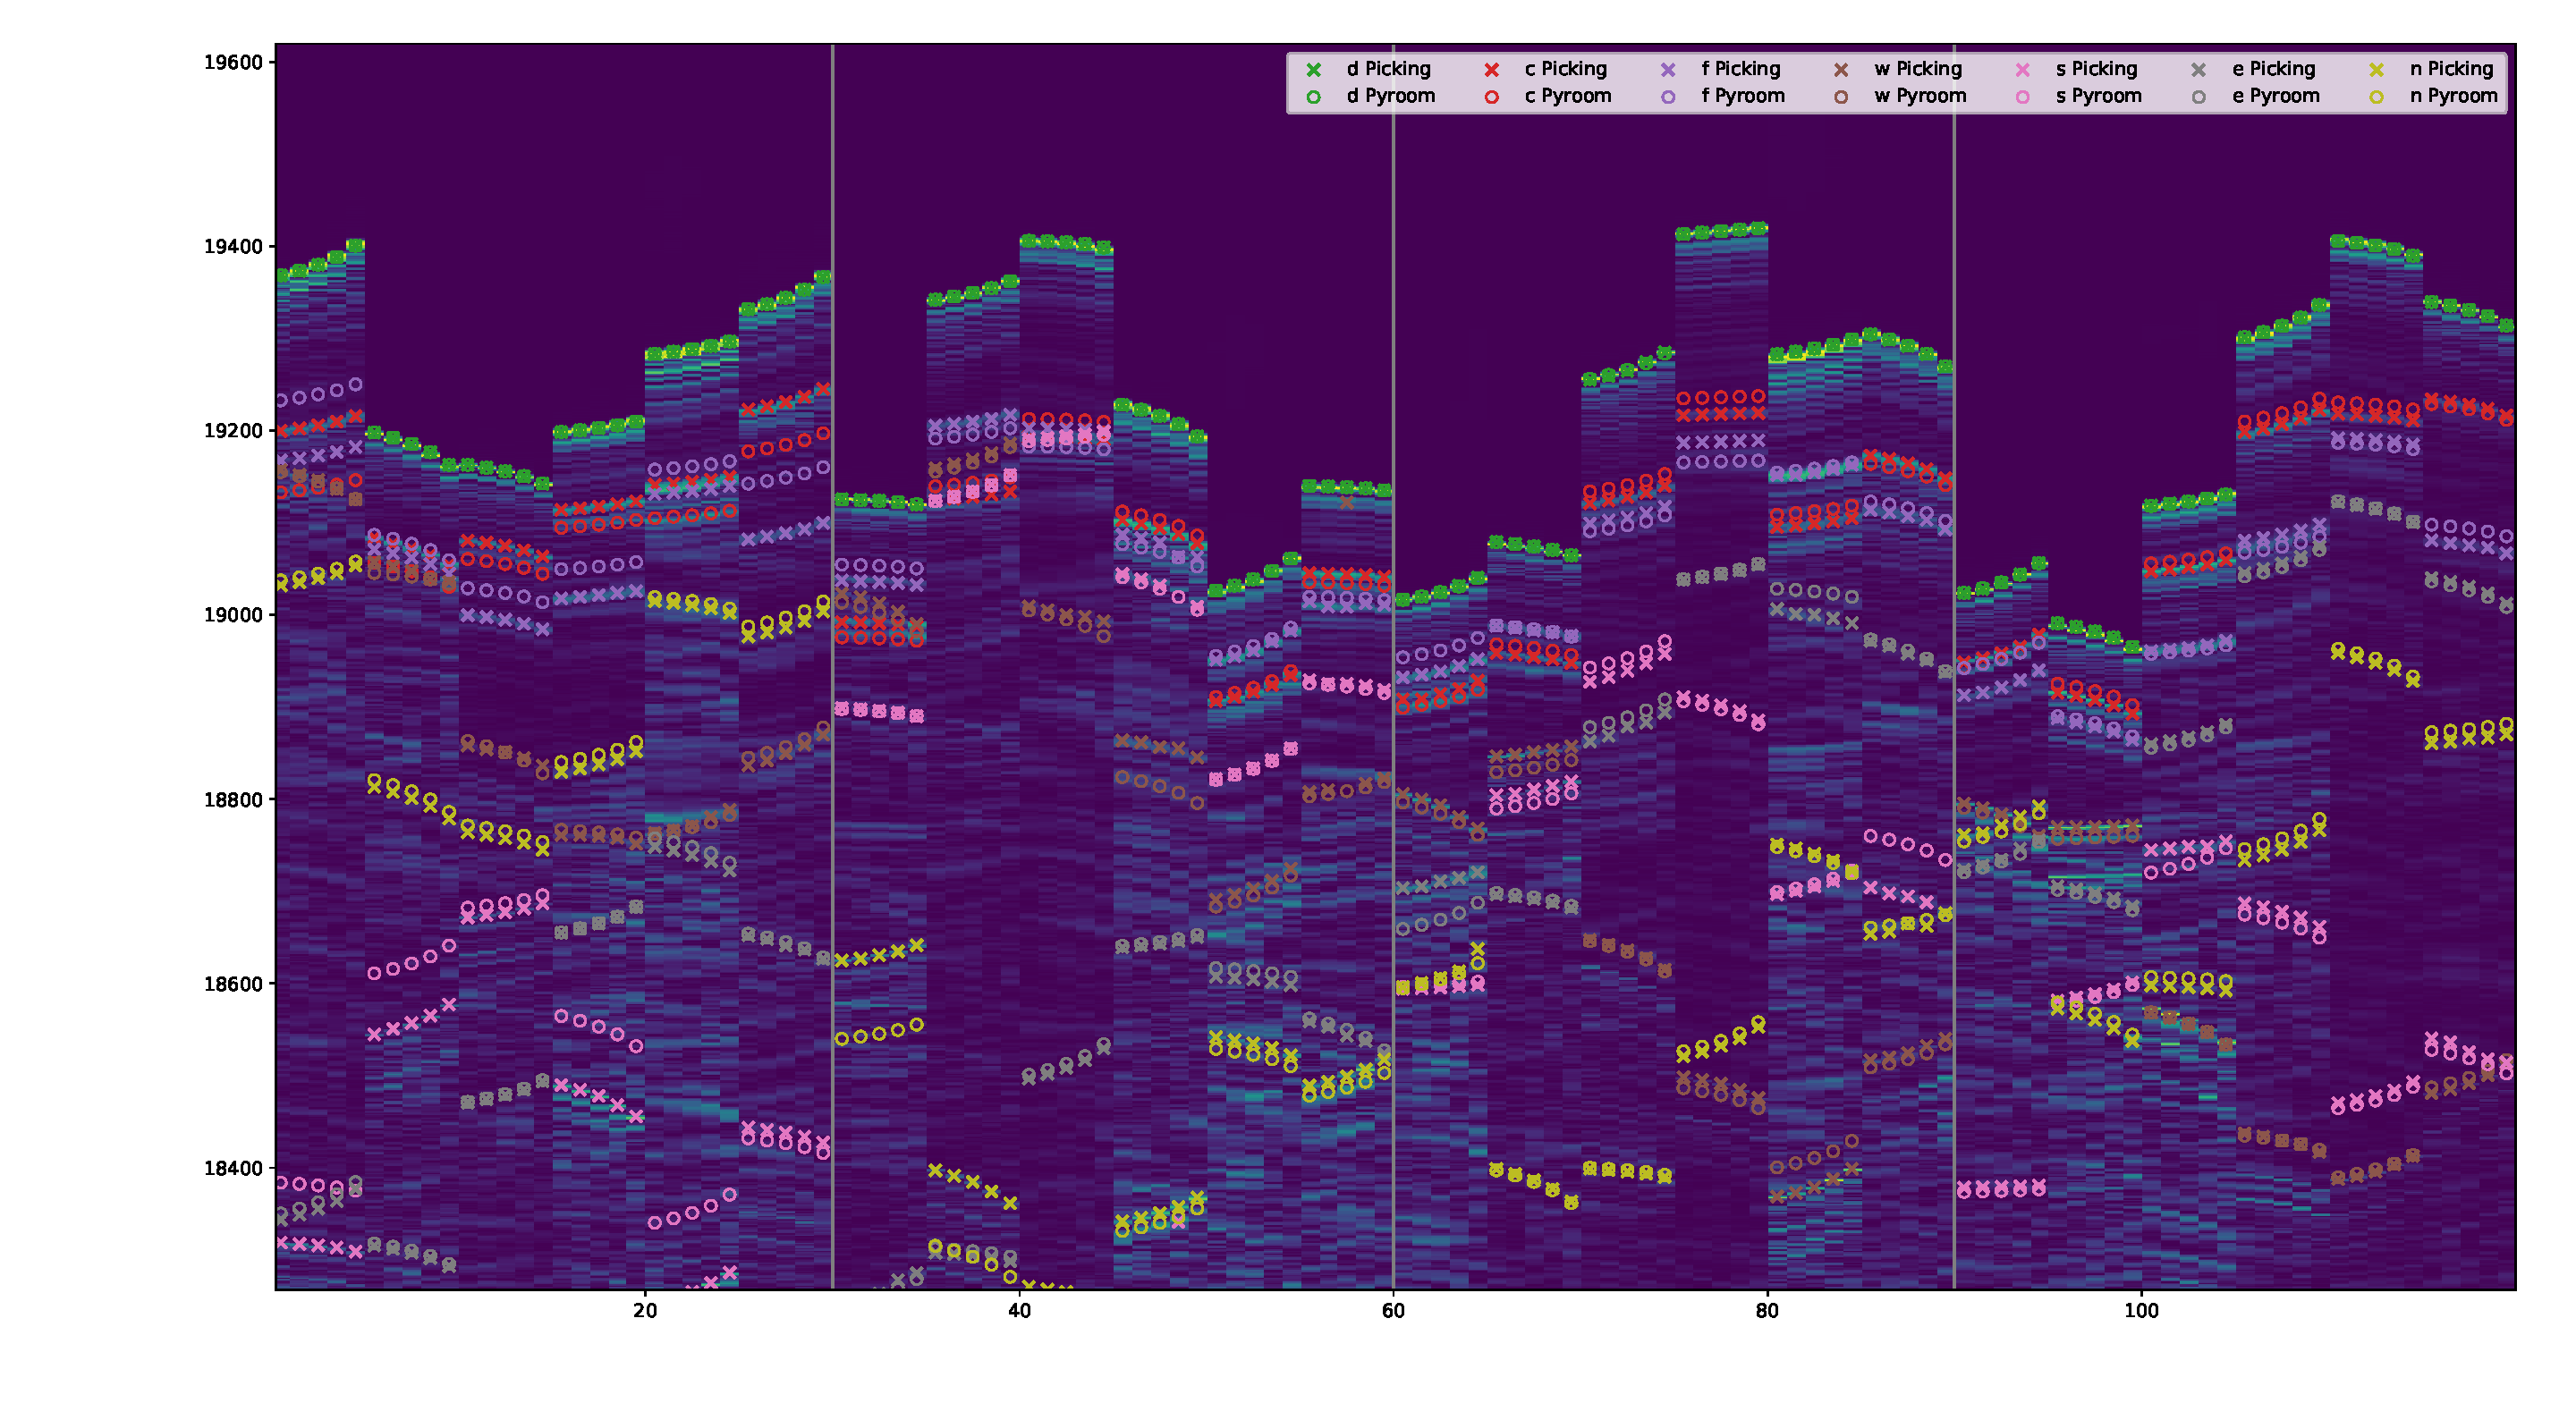
\includegraphics[trim={10em 0 0 0},clip,width=\linewidth]{figures/dechorate/rir_skyline_final_mod4paper.pdf}
    \end{center}
\end{frame}

\subsection{Application of \dechorate}

\begin{frame}[t]{Room Geometry Estimation (RooGE) with \dechorate}

    \begin{block}{}
        Estimating the room geometry: shape, volume or reflector position
        \\from signal or form TOAs and labels
    \end{block}

    \begin{block}{RooGE as \alert{Image Source Inversion}}
        If TOAs annotation (label and value) are available:
        \\For each wall/label:
        \begin{enumerate}
            \item TOA $\kto$ image source position via 3D multilateration
            \item image source position $\kto$ reflector estimation via geometric reasoning
        \end{enumerate}
    {\small \textcolor{gray}{other methods differ for priors and setup~\cite{filos2011robust,antonacci2012inference,crocco2017uncalibrated}}}
    \end{block}

    \only<2>{
        \begin{columns}
            \begin{column}{.48\textwidth}
                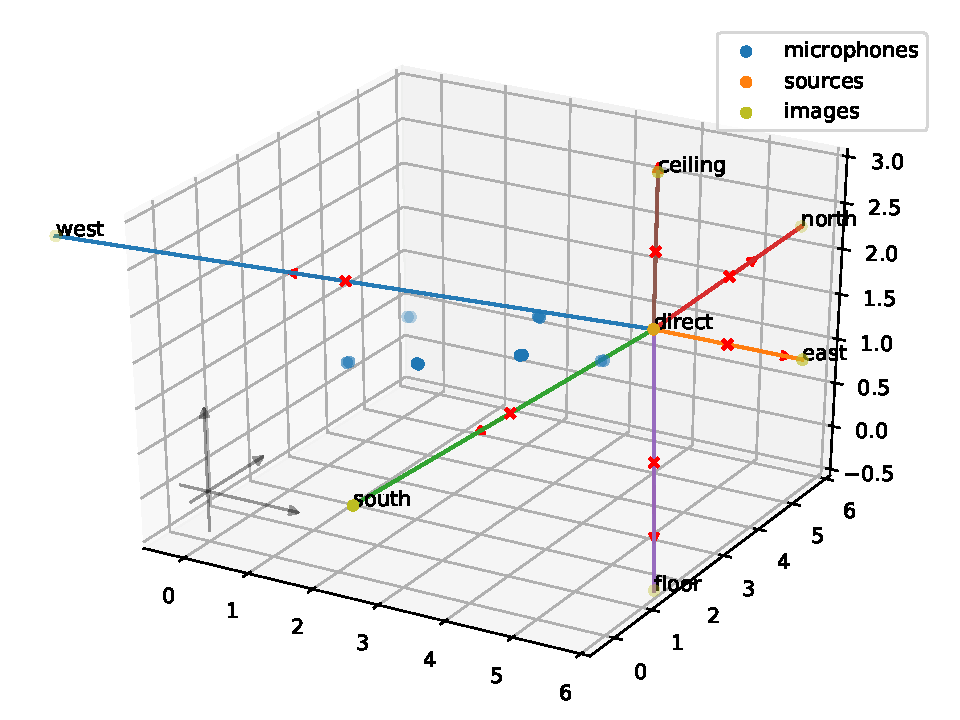
\includegraphics[width=\textwidth]{figures/dechorate/estimated_image}
            \end{column}\hfill
            \begin{column}{.48\textwidth}
                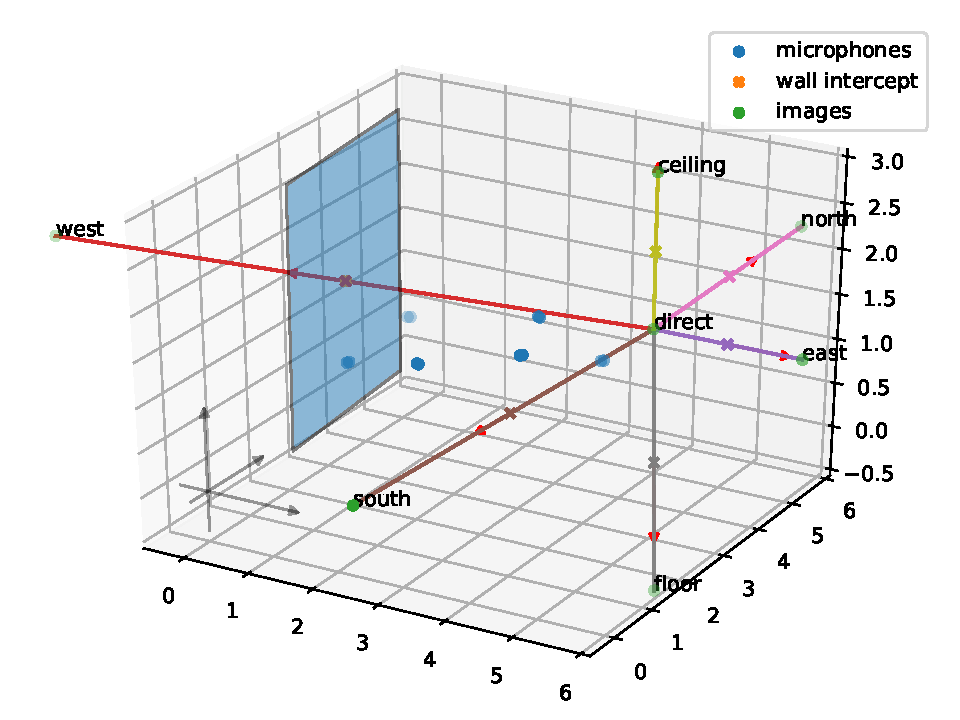
\includegraphics[width=\textwidth]{figures/dechorate/estimated_reflector}
            \end{column}
        \end{columns}
    }

    \only<3>{
        \begin{adjustbox}{minipage=.9\textwidth,margin=0pt \smallskipamount,center}
            \centering
            \small
            \begin{tabular*}{\linewidth}{c|cc|cc|cc|cc}
                \toprule
                source id &	1	& &	2	& &	3	& &	4 &	\\
                wall &	DE&	AE&	DE&	AE&	DE&	AE&	DE&	AE\\
                \hline
                west &	0.74	& $\ang{8.99}$      & 4.59	& $\ang{8.32}$  & 5.89	& $\ang{5.75}$	& $\mathbf{0.05}$    & $\mathbf{\ang{2.40}}$\\
                east &	$\mathbf{0.81}$	& $\mathbf{\ang{0.08}}$      & 0.9	& $\ang{0.50}$	&$\mathit{69.51}$	& $\mathit{55.70}^\circ$	& 0.31    & $\ang{0.21}$\\
                south&	3.94	&$\mathit{16.08}^\circ$      & $\mathbf{0.18}$	& $\ang{1.77}$	&$\mathit{14.37}$ & $\mathit{18.55}^\circ$	& 0.82    & $\mathbf{\ang{1.65}}$\\
                north&	1.34	& $\ang{0.76}$	    & 1.40	& $\ang{8.94}$	& $\mathbf{0.63}$	& $\mathbf{\ang{0.17}}$	& 2.08    & $\ang{1.38}$\\
                floor&	$\mathbf{5.19}$	& $\mathbf{\ang{1.76}}$	    & 7.27	& $\ang{2.66}$	& 7.11	& $\ang{2.02}$	& 5.22    & $\ang{1.90}$\\
                ceiling&1.16	& $\ang{0.28}$	    & 0.67	& $\ang{0.76}$	& $\mathbf{0.24}$	& $\ang{1.16}$	& $0.48$    & $\mathbf{\ang{0.26}}$\\
                \bottomrule
                \end{tabular*}
        \end{adjustbox}
        {\small \textcolor{gray}{Distance Error (DE) [cm] and Angular Error (AE)}}

    }

\end{frame}

\begin{frame}{Echo-aware Speech Enhancement}
    \begin{block}{Speech Enhancement}
        Improve the quality of a \textit{target} sound source with respect:
        \begin{itemize}
            \item interferences, i.e. form other sources $\rightsquigarrow$ sound source separation
            \only<1>{
            \item background noise $\rightsquigarrow$ denoising
            \item reverberation $\rightsquigarrow$ dereverberation, room equalization
            }
            \only<2>{
            \item \alert{background noise $\rightsquigarrow$ denoising}
            \item \alert{reverberation $\rightsquigarrow$ dereverberation, room equalization}
            }
        \end{itemize}
    \end{block}

    \begin{block}{Spatial filtering via Beamformers}
        \begin{itemize}
            \item Is a speech enhancement techniques for multichannel
            \item vs. Wiener Filtering, the target is distortionless
            \item in anechoic case, it correspond to delay-and-sum beamformer
            \item physical interpretation with steering vector based on DOA
            \item both in time and \only<2>{\alert{frequency}}\only<1>{frequency} domain
        \end{itemize}
    \end{block}

    \begin{mydefblock}{Beamformer: closed-form solution}
        \begin{equation*}
            \bfw = \kinv{\boldsymbol{\Sigma}_n} \bfC (\khermitian{\bfC} \kinv{\boldsymbol{\Sigma}_n} \bfC) \bfg
        \end{equation*}
    \end{mydefblock}


\end{frame}

\begin{frame}[t]{Echo-aware Speech Enhancement}

    \begin{block}{The PSD of various components}
        asd
    \end{block}

    \begin{block}{Different Criteria and Solution}
        \begin{itemize}
            \item DS
            \item MVDR - DP
            \item MVDR ReTF
        \end{itemize}
    \end{block}

    \begin{center}
        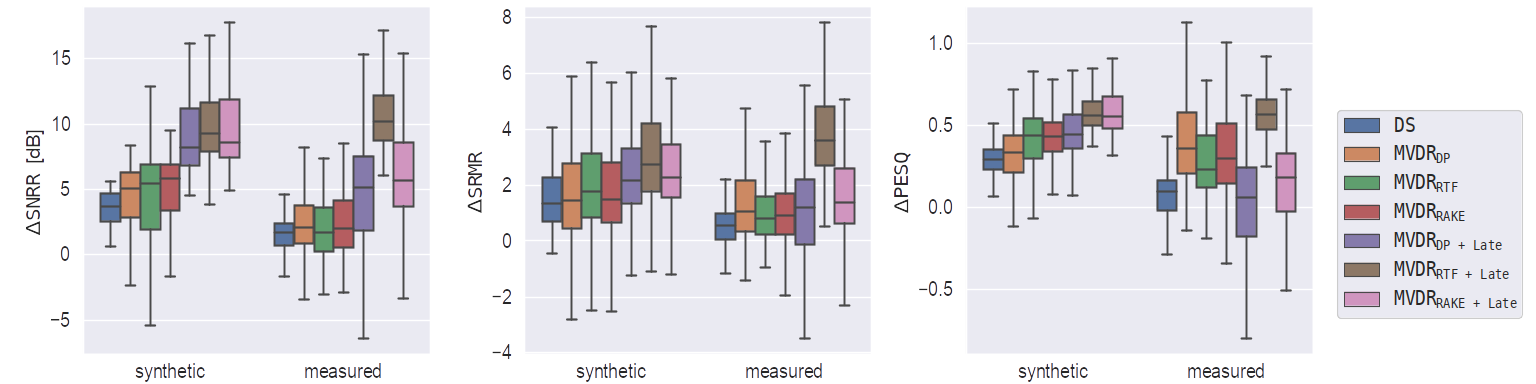
\includegraphics[width=\textwidth]{figures/dechorate/kowalkzy_results_boxplot_alpha.png}
    \end{center}

\end{frame}

% \subsection*{Interim conclusion (3/4)}

% \begin{frame}{Interim conclusion (3/4)}
%     \begin{block}{\dechorate dataset for echo-aware signal processing}
%         \begin{itemize}
%             \item designed for AER, SE and RooGE
%             \item Geometrical annotation $\longleftrightarrow$ image source annotation $\longleftrightarrow$ Signal Annotation
%             \item Measured Real RIRs and equivalent synt RIR
%             \item also speech, noise, babble noise and different room conf (+fornitures)
%             \item GUI, tools and code
%         \end{itemize}
%     \end{block}

%     \begin{block}{Application}
%         Echo Estimation
%         \begin{itemize}
%             \item Huge difference between real and simulated data
%         \end{itemize}
%         Room Geometry Reconstruction
%         \begin{itemize}
%             \item some annotation inconsistencies are noticed (but manually corrected)
%         \end{itemize}
%         Echo-aware Speech Enhancement
%         \begin{itemize}
%             \item a
%             \item b
%         \end{itemize}
%     \end{block}
% \end{frame}